\exercise

Given the following tree:
%
\begin{figure}[H]
  \centering
  \tikzstyle{level 1}=[level distance=1.2cm, sibling distance=1.5cm]
  \tikzstyle{level 2}=[level distance=1.2cm, sibling distance=1.25cm]
  \tikzstyle{level 3}=[level distance=1.2cm, sibling distance=1cm]

  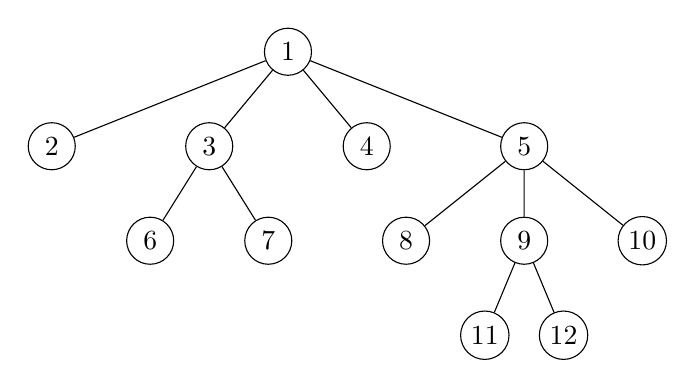
\begin{tikzpicture}[grow=down, sloped]
  \node[draw,fill=white, circle, inner sep=2pt, minimum size=17pt] {1}
  child {
    node[draw,fill=white, circle, inner sep=2pt, minimum size=17pt] {2}
    edge from parent[-]
  } child {
    node[draw,fill=white, circle, inner sep=2pt, minimum size=17pt] {3}
    child {
      node[draw,fill=white, circle, inner sep=2pt, minimum size=17pt] {6}
      edge from parent[-]
    }
    child {
      node[draw,fill=white, circle, inner sep=2pt, minimum size=17pt] {7}
      edge from parent[-]
    }
    edge from parent[-]
  } child {
    node[draw,fill=white, circle, inner sep=2pt, minimum size=17pt] {4}
    edge from parent[-]
  } child {
    node[draw,fill=white, circle, inner sep=2pt, minimum size=17pt] {5}
    child {
      node[draw,fill=white, circle, inner sep=2pt, minimum size=17pt] {8}
      edge from parent[-]
    }
    child {
      node[draw,fill=white, circle, inner sep=2pt, minimum size=17pt] {9}
      child {
          node[draw,fill=white, circle, inner sep=2pt, minimum size=17pt] {11}
          edge from parent[-]
      }
      child {
          node[draw,fill=white, circle, inner sep=2pt, minimum size=17pt] {12}
          edge from parent[-]
      }
      edge from parent[-]
    }
    child {
      node[draw,fill=white, circle, inner sep=2pt, minimum size=17pt] {10}
      edge from parent[-]
    }
    edge from parent[-]
  };
  \end{tikzpicture}
\end{figure}
%
\begin{enumerate}
  \item compute its LOUDS representation;
  \item compute the children of node 5;
  \item can we jump directly to its fourth child?
\end{enumerate}

\solution

\begin{enumerate}

  \item First, we have to place a dummy root node to the tree and, then, compute
  the degrees of each note, as in picture:
  %
  \begin{figure}[H]
    \centering
    \tikzstyle{level 1}=[level distance=1.2cm, sibling distance=2cm]
    \tikzstyle{level 2}=[level distance=1.2cm, sibling distance=1.5cm]
    \tikzstyle{level 3}=[level distance=1.2cm, sibling distance=1cm]

    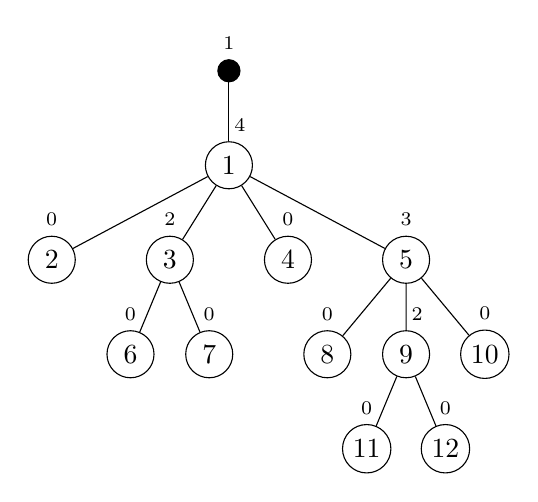
\begin{tikzpicture}[grow=down, sloped]
    \node[draw,fill=black, circle, inner sep=2pt, minimum size=8pt, label={\scriptsize 1}] {}
    child {
      node[draw,fill=white, circle, inner sep=2pt, minimum size=17pt, label={\scriptsize \quad 4}] {1}
      child {
        node[draw,fill=white, circle, inner sep=2pt, minimum size=17pt, label={\scriptsize 0}] {2}
        edge from parent[-]
      } child {
        node[draw,fill=white, circle, inner sep=2pt, minimum size=17pt, label={\scriptsize 2}] {3}
        child {
          node[draw,fill=white, circle, inner sep=2pt, minimum size=17pt, label={\scriptsize 0}] {6}
          edge from parent[-]
        }
        child {
          node[draw,fill=white, circle, inner sep=2pt, minimum size=17pt, label={\scriptsize 0}] {7}
          edge from parent[-]
        }
        edge from parent[-]
      } child {
        node[draw,fill=white, circle, inner sep=2pt, minimum size=17pt, label={\scriptsize 0}] {4}
        edge from parent[-]
      } child {
        node[draw,fill=white, circle, inner sep=2pt, minimum size=17pt, label={\scriptsize 3}] {5}
        child {
          node[draw,fill=white, circle, inner sep=2pt, minimum size=17pt, label={\scriptsize 0}] {8}
          edge from parent[-]
        }
        child {
          node[draw,fill=white, circle, inner sep=2pt, minimum size=17pt, label={\scriptsize \quad 2}] {9}
          child {
              node[draw,fill=white, circle, inner sep=2pt, minimum size=17pt, label={\scriptsize 0}] {11}
              edge from parent[-]
          }
          child {
              node[draw,fill=white, circle, inner sep=2pt, minimum size=17pt, label={\scriptsize 0}] {12}
              edge from parent[-]
          }
          edge from parent[-]
        }
        child {
          node[draw,fill=white, circle, inner sep=2pt, minimum size=17pt, label={\scriptsize 0}] {10}
          edge from parent[-]
        }
        edge from parent[-]
      }
    };
    \end{tikzpicture}
  \end{figure}
  %
  We now construct its LOUDS representation by concatenating the degrees of each
  node (from top to bottom, from left to right), expressed in inverse unary:
  %
  \begin{align*}
    B = \overbracket[0pt][1pt]{10}^{root}\ \overbracket[0pt][1pt]{11110}^{1}\
    \overbracket[0pt][1pt]{0}^{2}\ \overbracket[0pt][1pt]{110}^{3}\
    \overbracket[0pt][1pt]{0}^{4}\ \overbracket[0pt][1pt]{1110}^{5}\
    \overbracket[0pt][1pt]{0}^{6}\ \overbracket[0pt][1pt]{0}^{7}\
    \overbracket[0pt][1pt]{0}^{8}\ \overbracket[0pt][1pt]{110}^{9}\
    \overbracket[0pt][1pt]{0}^{10}\ \overbracket[0pt][1pt]{0}^{11}\
    \overbracket[0pt][1pt]{0}^{12}\
  \end{align*}
  %
  In this array, the $i$-th node is represented by the $i$-th 1 in the sequence,
  while its children correspond to the 1s following the $i$-th 0 (so, every node
  is represented \emph{twice}).

  \item We cand find the children of the $i$-th node (in this case, $i = 5$)
  using a $Select_0$ data structure in the following way:
  %
  \begin{enumerate}

    \item we compute the index of the first bit after the fifth 0, with
    $$y = Select_0(B, i) + 1 = Select_0(B, 5) + 1 = 13;$$

    \item we compute the $id$ of the child at position $y$ with $$Rank_1(B, y) =
    Select_0(B, i) - i = y - i = 8;$$

    \item we search for the next sibling by scanning the next bit in the array
    ($y = y + 1$) and repeating the procedure from step (b) until we find that
    $B_y = 0$, then we have finished.

  \end{enumerate}

  \item No, we have to scan the children bit-by-bit or check if the node has at
  least 4 children by computing its degree with
  $$degree(i) = Select_0(B, i + 1) - Select_0(B, i) - 1.$$
  In this case, $degree(5) = 3 < 4$, so we can not jump to its fourth child.

\end{enumerate}
